\def\DevnagVersion{2.15}\documentclass[a4paper, 11pt, notitlepage]{report}

\usepackage{amsfonts} 
\usepackage[english]{babel}
\usepackage{amsmath}
\usepackage{graphicx} % if you want to include jpeg or pdf pictures
\usepackage{devanagari}
\usepackage{xcolor}
\usepackage{hyperref}
\usepackage{capt-of}
\usepackage{geometry}
\geometry{
    body={6.0in,9.5in},
    left= 1.0in,
    top = 0.5in}

\usepackage{hyperref}
\hypersetup{
    colorlinks,
    citecolor=black,
    filecolor=black,
    linkcolor=blue,
    urlcolor=black
}
\usepackage{color}
\definecolor{gray1}{RGB}{192,192,192}
\definecolor{gray}{RGB}{240,240,240}  
  
\author{Diwakar Chauhan} % change this
\date{\today} % change this

\begin{document}

\begin{center}
%\renewcommand{\rmdefault}{ptm}

{\color{blue} \fontfamily{rmdefault} \textsc{\LARGE IIT Kanpur}\\[1.5cm] }
\textsc{\Large B.Tech Project}\\[1cm]
\hrule height 2pt
\vspace*{10pt}
%\end{center}
{\huge  Language Independent Noun and Verb Acquisition from Psychological Videos}\\[0.4cm] 
\hrule height 2pt 
\vspace*{10pt}
%\\[1cm]
\begin{minipage}{0.4\textwidth}
\begin{flushleft} \large
\emph{Author:}\\
{\color{blue} \href{http://home.iitk.ac.in/~diwakarc}{Diwakar Chauhan} }
\end{flushleft}
\end{minipage}
\begin{minipage}{0.4\textwidth}
\begin{flushright} \large
\emph{Supervisor:} \\
{\color{blue} \href{http://www.cse.iitk.ac.in/users/amit}{Prof. Amit Mukerjee } }% Supervisor name - remove the \href bracket to remove the link  
\end{flushright}
\end{minipage}\\[3cm]


{\large \today}\\[4cm] % Date

\end{center}

\thispagestyle{empty}

\newpage
\section*{Acknowledgements}

\hspace*{30pt} This project is completed direct or indirect help of many people. I want to thank them all for their support.\\

\hspace*{10pt} I am thankful to my project supervisor for guiding me through this project.Due to his sincere and timely guidance, I was able to do this project.\\

\hspace*{10pt} Many-many thanks to Dr. Uta Frith, Institute of Cognitive Neuroscience, University College London, and  her Ph.D student Sarah White for providing me with psychological videos which were the core of the project.\\

\hspace*{10pt} I am thankful to Mr. Sushobhan Nayak for his work on language acquisition. This helped me a lot in the project.\\

\hspace*{10pt} I am also thankful to Mr. Prashant Jalan for doing syllable based noun discovery on the same video. Syllable based analysis helped to understand more about the co-relation of objects with utterances. He helped me in collecting the commentaries and transcribing to text.

\tableofcontents 

\newpage
%%%%%%%%%% MAIN TEXT STARTS HERE %%%%%%%%%%
\hspace*{10pt} \section*{Abstract}

In Natural language processing and learning, the process of language acquisition can be modeled as similar to the learning process of an infant.  The reason of this assumption is that, in both of the processes, there is very less or nothing prior knowledge about language or any other thing. The children across the world start learning their native language at almost same age\cite{EngJapChi}. They start from simple linguistic units and then learn complex ones later on. In all this development process, the children learning different languages are have very less age difference between them.
\hspace*{15pt} Therefore modeling language acquisition as similar process to the child learning, gives us freedom to generalize for multiple languages. We apply this process two major language spoken in India i.e. Hindi and English. These two languages represent two very different classes of languages. Hindi is much more inflected language as compared to English and English has large set of lexemes. In Hindi there are much more variations of lexemes in order to represent different parts of speech, gender and tense. Therefore learning identification usage of a single word is a non trivial task. In such situations syllable based results may give better results compared to lexeme based. While English has larger set of words mapping to same image schema. Therefore identifying words corresponding to a image schema is also a non trivial task.\\
Here we try to get the mapping of words with image schemas in both of the languages.\\

%%%%%%%%%%%%%%%%%%%%%%%%%%%%%%%%%%%%%%%%%%%%%%%%%%%%%%%%%%%%%%%%%%%%

%%%%%%%%%% SAMPLE CHAPTER %%%%%%%%%%
\chapter{Introduction}
\hrule height 2pt
\vspace*{10pt} 

\hspace*{10pt} \section{Human Learning Process :}
In the language learning process, humans start with learning identity of the objects i.e. nouns. Further they learn, the relationship between the object i.e. prepositions and interaction of objects i.e. verbs. The language mapping to the visual sequences can be formalized\cite{ICDICD544} as : \\
\hspace*{50pt}{\bf 1 - } Language learning objective is to map $S$ to $I$.\\ 
\hspace*{50pt}{\bf 2 - } Set of points in $S$ and $I$ are the training set.\\\\
where\\
\hspace*{40pt}$S$ is the language space\\
\hspace*{40pt}$I$ is the image sequence space\\

Nouns are learned before the verbs because objects require very less information as compared to the actions. The reason behind this may be that verbs therefore activities, require more information. 
The infants have no prior knowledge about the environment. They see shapes, faces and moving objects in in front of them. At the same time they hear utterances of the people. The utterances spoken around the child are usually proper sentences. These contain diverse range of words. But there are some words which are specific to that particular object or action. Initially the kids don't know the word boundaries. So they try to map the phonetics of utterances with the visual sequences. Once they know the word boundaries, they map words to the visual sequences. So in both ways they filter out the words specific to visual sequences out of all the utterance and ignore the common or irrelevant words. Naigles(1990)\cite{naigles} demonstrated that while learning meaning of verbs, infants use the syntactic information. She proved that given a illegal verbs in a sentence the children use the syntax to guess the meaning of the verb. \\

\begin{figure}[h]
\center
\begin{tabular}{c}
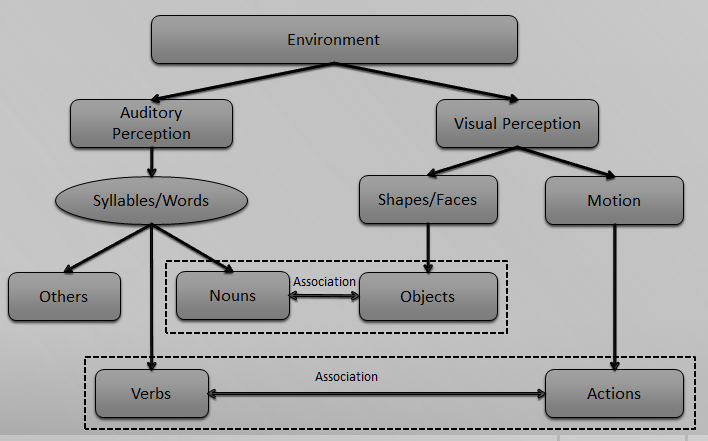
\includegraphics[scale=0.5]{childLearn1.png}
\end{tabular}
\label{tab:gt}
\caption{The schematic of learning process of child}
\end{figure}


However difficult the learning process of infants may be, they do not analyze large amount of data in order to learn the meanings of verbs or recognize the activities. They learn from the competent speakers who know to relate the words to the event's objects in the environment.\cite{kerr-cohen-08_wubble-world-lang-acquisition} And the children can extend their learning from one event to another. 

Here we are trying to understand the learning process of infant and based on that learning process, try to discover actions in psychological videos and map Hindi and English verbs to them. The application of this process of multiple language shows that this process is independent of the language being learned.



\section{Actions} 
\hspace*{10pt} Actions can be based on the the variations in the shape and size change , poses\cite{pami-Ben-ArieWPR02}  or orientation of the object. For example a person walking can be identified by motion of his hands and legs relative to his body\cite{JacksonBP05}. Similar can be said about the actions involving multiple agents. But what if the action which either don't need any shape changes to be expressed or the agent is an abstract object. These type of actions are represented either by specific motion of single object or particular type of motions and interaction between the agents. In this project we analyze the second type of actions.\\
%%place samples from the video

\section{Psychological Videos :}
\hspace*{10pt} Psychological videos are most used videos for study cognitive learning. These type of videos are manually created. The position of the objects in each of the frame of the video is result of the complex cognitive process of human mind. Each frame is designed to be a part of representation of some goal. Therefore the motion of the objects in these videos have some intent. This property of being simplistic in representation and complex in aim makes them very useful for machine learning and natural language processing purposes.\\
One of the very well known and widely studied psychological videos is Heider Simmel \cite{heider} video. In this video, there is a big box with a door, a small circle and two square shapes of different sizes. The actions represented in this video are {\bf Chase}, {\bf Go Away} and {\bf Come Closer}.

\begin{figure}[h]
\center
\begin{tabular}{ccc}
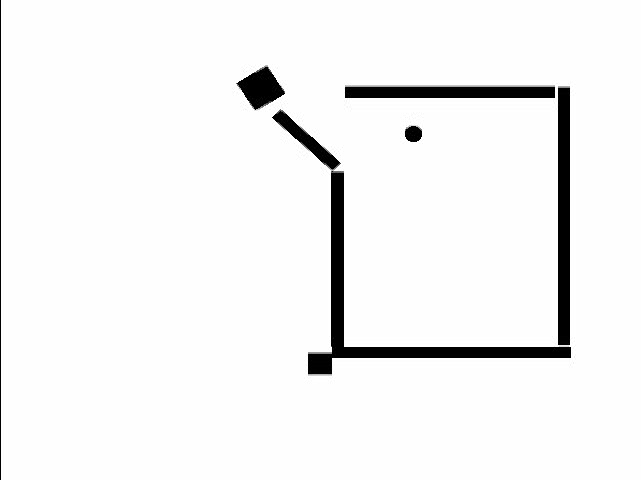
\includegraphics[scale=0.15]{image/heider1135.png} &
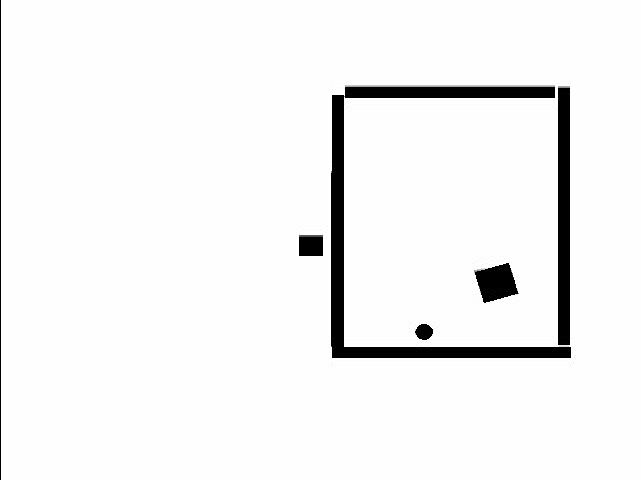
\includegraphics[scale=0.15]{image/heider1345.png} &
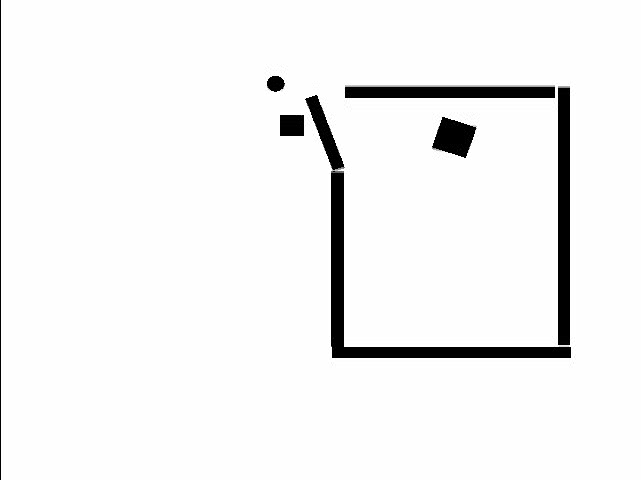
\includegraphics[scale=0.15]{image/heider1810.png}
\end{tabular}
\label{tab:gt}
\caption{Stills from Heider Simmel video}
\end{figure}

With this video, only the above described actions can be learned. For other type of actions and more complex actions, we needed some dataset which contains variety of actions. One appropriate choice for this purpose is animations from Frith-Happe\cite{fhanimation}\\

\hspace*{10pt} These animations contain only two dynamic agents which are triangles. Each of the the videos represents a particular simple or complex transitive action. By complex action we mean that the action constitutes smaller actions, e.g. the "Coxing" in the video consists of many instances of {\dn D\3C3wA d\?nA} and {\dn \8{G}mnA}. Then action discovery is done in two ways:- \\

\subsection{Completely Unsupervised Action Discovery :}

Here we start with zero information about the video or the actions in it. We take one videos and apply HMM  on the feature vectors extracted from the frames of video. We take frames in small consecutive groups. We create HMM for each of this groups and evaluate the mutual acceptance measure for each of the groups. Based on this measure, hierarchical clustering is done and cluster tree is generated. This cluster tree is later cut at some point to produce some clusters. These clusters are action classes.\\

\subsection{User labeled Action Discovery :} 

We label the video with actions occurring in video. Not we learn HMM on each of the user labeled action cluster. Then we merge the most similar clusters using mutual acceptance of HMM \hyperref[sec:distHMM]{(section \ref*{sec:distHMM})} . On theses clusters, the associated commentaries are calculated. We calculate the relative frequency measure for words in a cluster. After that remove nouns and common words to get the verbs for the clusters.\\

\subsection{Noun Discovery : } At the same time commentary is taken for the video. This commentary is processed to remove less important words. Then we take the part of commentaries which are more relevant to the triangles using attention model. And then we calculate association measures for each of the remaining words. Based on this association measure, the nouns are identified.\\

Below is the schematic of the whole process used in the project :-

\begin{figure}[h]
\center
\begin{tabular}{c}
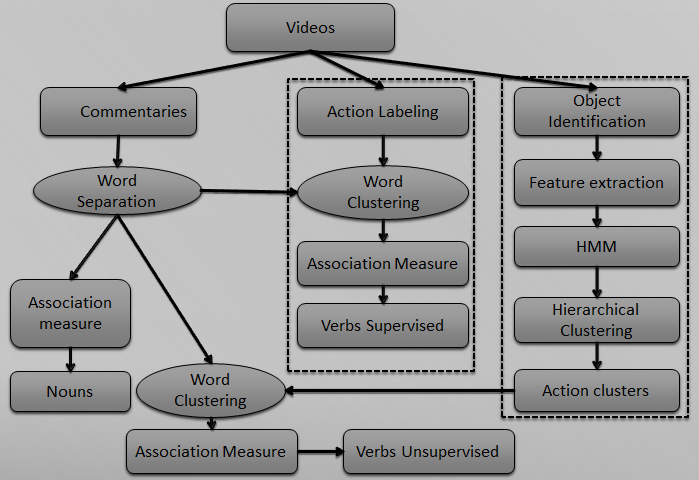
\includegraphics[scale=0.5]{schematic1.png}
\end{tabular}
\label{tab:gt}
\caption{The schematic of the whole process}
\end{figure}

%%%%%%%%%%%%%%%%%%%%%%%%%%%%%%%%%%%%%%%%%%%%%%%%%%%%%%%%%%%%%%%%%%%%%%%%%%%%%%%

%%%%%%%%%%%%%%%%%%%%%%%%%%%%%%%%%%%%%%%%%%%%%%%%%%%%%%%%%%%%%%%%%%%%%%%%%%%%%%%%%%
\chapter{Vision and Language Dataset }
\hrule height 2pt
\vspace*{10pt} 
In order to recognize the actions and corresponding language labels for the language, we need proper datasets of visual sequences as well as language. The visual dataset should be something which contains various type of actions clearly represented. And similarly language database for the visual sequences should be correctly aligned to the visual sequences.

\section{ Visual Database :} The video used in this project are psychological videos. These videos were made by Dr. Uta Frith. She is a professor at Institute of Cognitive neuroscience, University of London. These videos were initially created for the purpose of identification of Autism in children and their further evaluation. There are three classes in the dataset, each containing 4 videos : \\
\hspace*{10pt}{\bf 1- GD :} This class contains videos with goal directed actions.The videos in this class are chase,dance, fight, lead.\\ 
\hspace*{10pt}{\bf 2- TOM :} This class contains videos testing Theory of Mind. The videos in this category are coax, mock, seduce, surprise.\\
\hspace*{10pt}{\bf 3- Random :} In this class the videos represent random actions likely drift, billiard, star, tennis.


\begin{figure}[h]
\center
\begin{tabular}{ccc}
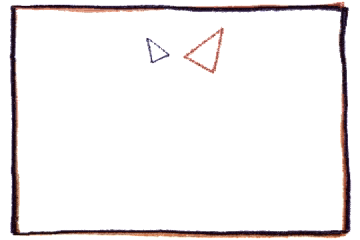
\includegraphics[scale=0.3]{sample65dance.png} & 
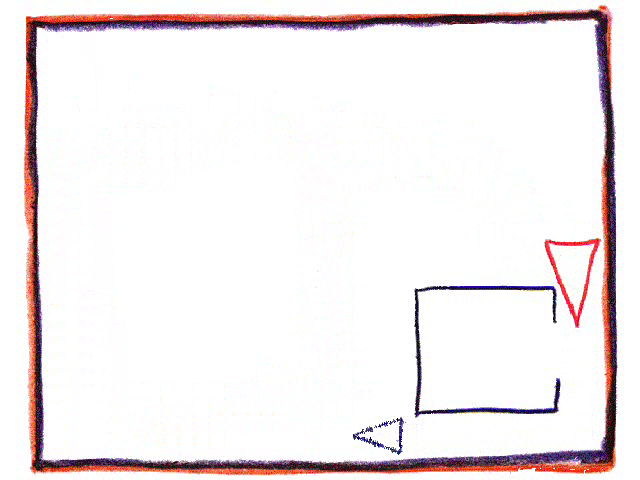
\includegraphics[scale=0.15]{sample174chase.png} &
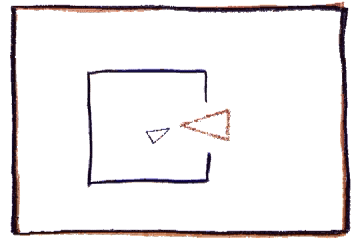
\includegraphics[scale=0.3]{sample198coax.png}
\end{tabular}
\label{tab:gt}
\caption{Stills from animations (a) Dancing Video, (b) Chase Video and (c) Coaxing Video }
\end{figure}


We recognised action clusters for chase and coax videos. The language modelling is done for the coaxing video due to its rich content of actions.
\subsection{Motion Data of objects in the video :}
In the videos we need to get the motion data of the objects in it. Motion data involves the frame intervals in which a particular object is moving and when it is not moving. Since in our videos only the triangles move, we need the motion data of these two triangles. This data is further used in recognition of nouns and verbs subsequently.

\hspace*{10pt} \section{Language Database : } Language database is created by manually taking the commentaries for the videos and then transcribing them into text. We took commentaries in two languages primarily for one video 'Coaxing'. $22$ commentaries in Hindi and $8$ commentaries in English.

\subsection{Collecting Commentaries :} Different people were asked to give commentary on the video. One subject could give at most on commentary in each of the language. Each subject was shown the video multiple times before giving the commentaries. The purpose of showing the video before commentary was to make the subject familiar with the environment. This would help him to speak simultaneously with the actions in the video at the time of giving the commentary.\\
\hspace*{10pt} Each subject was given certain instructions about the commentary. The instructions are as follows :-\\
{\it 
\hspace*{10pt} 1 - Describe the objects in the video and their interactions.\\
\hspace*{10pt} 2 - Do not involve yourself or any other external object as agent in the video.\\ 
\hspace*{10pt} 3 - Do not metaphorize the sentences, explain them as they appear. \\
\hspace*{10pt} 4 - Try to speak simultaneously \\
}
The subjects showed huge variety in their description of the video. Majority of the subjects considered the two triangles and the one side opened rectangular box. But some of subjects considered the rectangular shape enveloping all other objects as another object. Therefore their narration consisted of $4$ agents. Most of the subjects were stuck on their initial notion of the objects in the video, e.g. If a subject refers the larger triangle(also the red one) as {\dn bXA E/\7{B}\qq{j}} then he continues to refer it as this word only in the whole commentary and if he refers it as {\dn lAl E/\7{B}\qq{j}} then he does it in whole video. Very a few subjects mixed these words.  \\
After recording the commentaries, the audio files were embedded the the video. For each of the subject and language, a separate video was created with equal frame rate with the original animation video.\\

\begin{figure}[h]
\center
\begin{tabular}{c}
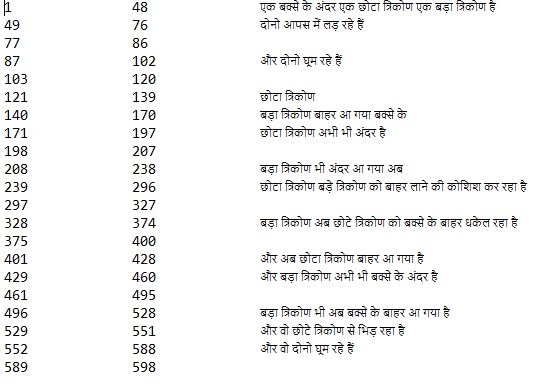
\includegraphics[scale=0.70]{comm.png}
\end{tabular}
\label{tab:gt}
\caption{Transcribed text for Hindi commentary}
\end{figure} 

\subsection{Transcribing to text :}
We did manual transcription of the commentaries. We followed a common procedure for transcribing commentaries of both the languages. The minimal unit of transcription was words. The words were separated from each other by spaces. The morphological variations of the words were kept as they were spoken. The small grammatical errors were corrected.\\
Now the utterances were divided into sentences or phrases. The basis of division was the length of sentences or phrases and the pauses made by the subject. If a sentence was larger than some predefined length and could be broken into two parts, we wrote it in two parts. Or if the subjects pauses for more than $5$ frames before uttering next words, we consider it in next line. The pauses of less than $5$ frames were bound to accuracy of measurement.\\

\begin{figure}[h]
\center
\begin{tabular}{c}
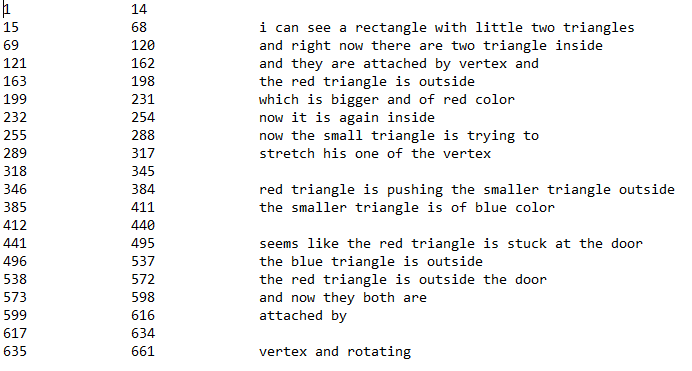
\includegraphics[scale=0.70]{commEng.png}
\end{tabular}
\label{tab:gt}
\caption{Transcribed text for one English commentary}
\end{figure} 

%%%%%%%%%%%%%%%%%%%%%%%%%%%%%%%%%%%%%%%%%%%%%%%%%%%%%%%%%%%%%%%%%%%%%%%%%

\chapter{Prelinguistic Image Schemata}
%\vspace*{5pt}
\hrule height 2pt
\vspace*{10pt}
Before mapping the language to visual sequences, we need to get the properties of the visual sequences : \\
\section{Agents in the psychological videos}
\hspace*{30pt} A sentence in a language consists of small units of words, phrases appearing as different parts of speech for that language. Theses different words are mapped to different image schema. The image schema can be considered as combination of two things. First is the objects participating in the image schema. Second is the feature vectors of the set of frames constructing the image schema. The function associating the feature vectors of the frames is the characteristic of the given image schema. Here we consider mainly two type of such schema i.e. for nouns and verbs. The nouns are used for the shapes occurring in the video. The prepositions are used for the relation objects . The verbs are used for interaction of the objects in the video and their motions.\\

\hspace*{10pt} To get such image schema, we needed data which has identifiable objects and their actions. So we use Frith-Happe \cite{fhanimation} animations. In these videos the objects are red triangle({\bf [RT]}, also the bigger triangle), blue triangle({\bf [BT]} also the smaller triangle) and a rectangular box {\bf [RB]}. The rectangle is static at specific position in all the frames. The two triangles move inside a frame. Through their motion, they represent various actions.\\

\begin{figure}[h]
\center
\begin{tabular}{ccc}
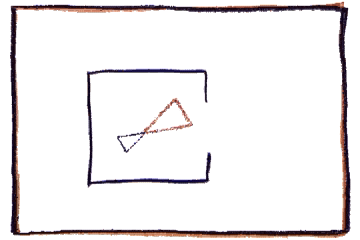
\includegraphics[scale=0.3]{image/0062.png} & 
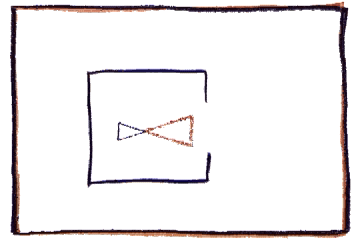
\includegraphics[scale=0.3]{image/0063.png} &
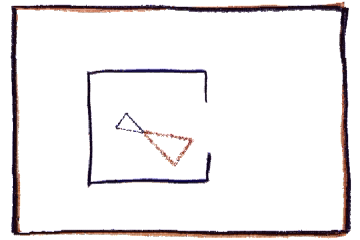
\includegraphics[scale=0.3]{image/0068.png}\\

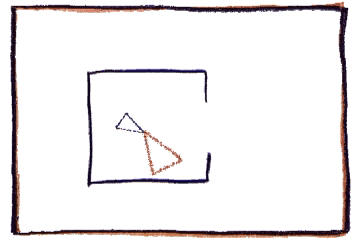
\includegraphics[scale=0.3]{image/0072.png} & 
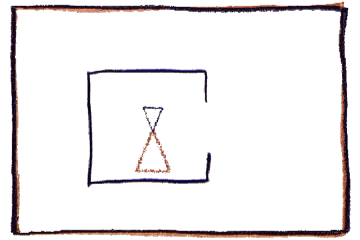
\includegraphics[scale=0.3]{image/0074.png} &
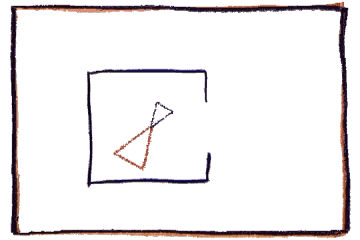
\includegraphics[scale=0.3]{image/0078.png}\\
\end{tabular}
\label{tab:gt}
\caption{The images representing the states of the triangles from Frame 62 to Frame 78 in the coaxing video. This image schema correspond to circling as spoken by most of subjects.}
\end{figure}

\begin{table}[h]
\begin{center}
\begin{tabular}{|c|c|p{8cm}|}
\hline
\multicolumn{1}{|c|}{Subject} & \multicolumn{1}{|c|}{Interval} & \multicolumn{1}{|c|}{Commentary} \\
\hline
Subject1 &51-89 &{\dn ek CoVA E/\7{B}j aOr ek bwA E/\7{B}j aAps m\?{\qva} K\?l rh\? h\4{\qva} } \\
\hline
Subject2 & 60-83 & {\dn ek \7{d}sr\? ko pkw kr \8{G}m rh\? h\4{\qva}}\\
\hline
Subject3 & 58-128 & {\dn lAl E/\7{B}j aOr ek nFlA E/\7{B}j dono ek \7{d}sr\? kA EsrA pkw kr \8{G}m rh\? h\4{\qva}}\\
\hline
\end{tabular}
\caption{The commentaries from the different subject on the at the time of the frames show above. The time interval of these commentaries completely contain the interval of the frames shown}
\end{center}
\end{table}

\hspace*{10pt} \section{Extracting Objects: }
We selected $4$ of the videos namely Coaxing and Chase to use in our project. In these videos there were three objects, a red triangle, a smaller blue triangle and and a rectangular box. In the rest of the two videos the rectangular box is absent.\\
The frames are converted to gray scale and following steps are done :\\
\\ \hspace*{10pt} In the first step, we determine the two triangles in the video and track them by background subtraction. To do so one frame of the video is taken as the base frame $fr_0$ and for each of frames $fr_i$, we calculate the difference of frames $d_i$ :
	$$d_i = fr_i - fr_0$$
Then we apply erosion and dilation to remove the noise in the image. At this step the triangles are not separated from each other but they are separated from rest of the static objects in the video. We use various image processing techniques to separate the triangles which are described below.
\hspace*{10pt} The triangles are made of lines segments. Therefore the most obvious way of determining a triangle is to determine it's edges. Hough transform is a very effective way of identifying the line segments in a data.\\

\subsection{Separation of the triangles}
\hspace*{10pt} In the video the sizes of both the triangles are significantly different. We take the benefit of f this difference. The line segments corresponding to the bigger triangle will have high intensity in the $(R, \Theta)$ space compared to that of the smaller triangle.\\
\hspace*{10pt} We take top three peaks in the $(R, \Theta)$ space and get the points corresponding to them in $(X,Y)$ space. These points form the bigger triangle. Once the line of a single triangle has been extracted, we can easily get its vertices by calculating the intersection points of the lines.\\
\hspace*{10pt} After separating the larger triangle, we apply same Hough Transform technique in the remaining points to get the edges of the smaller triangle and vertices subsequently.\\

\begin{figure}[h]
\center
\begin{tabular}{cc}
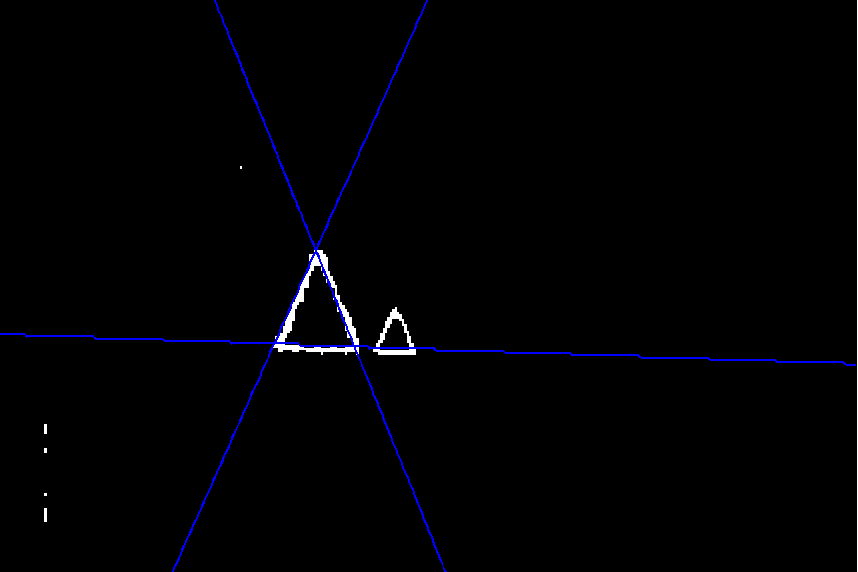
\includegraphics[scale=0.30]{0002l.png} & 
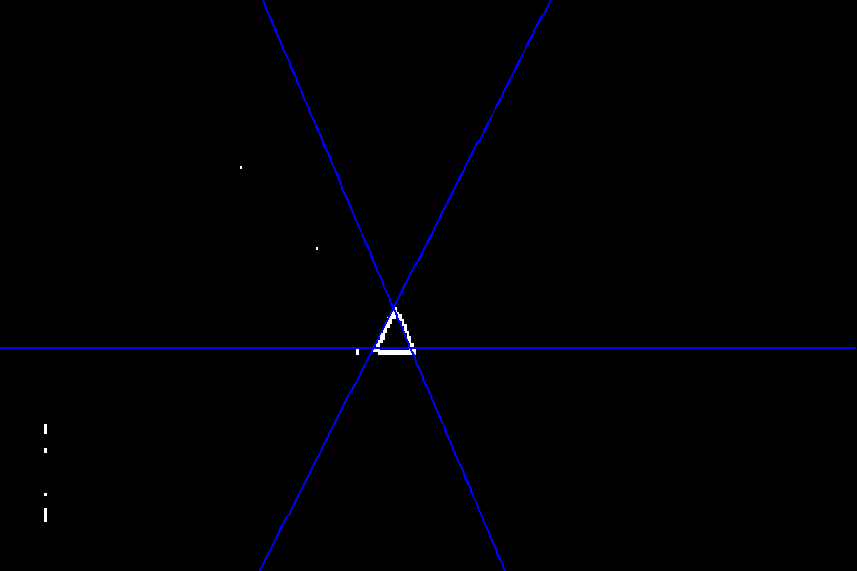
\includegraphics[scale=0.30]{0002s.png}
\end{tabular}
\label{tab:gt}
\caption{Two triangles as detected by Hough Transform}
\end{figure}

\subsection{Determination of the Rectangle }
Since the rectangle is static in the video. We can determine it in just one frame. After the triangles are identified and separated from the frame, we remove the white background and the black-red boundary. Then we are left with the points corresponding rectangle. On these points, applying hough transform, the four edges of the rectangle are determined. The four vertices of the rectangle are determined by intersection of the edges. And the vertices of the opening in the rectangle is determined by linear interpolation.\\
\begin{figure}[h]
\center
\begin{tabular}{c}
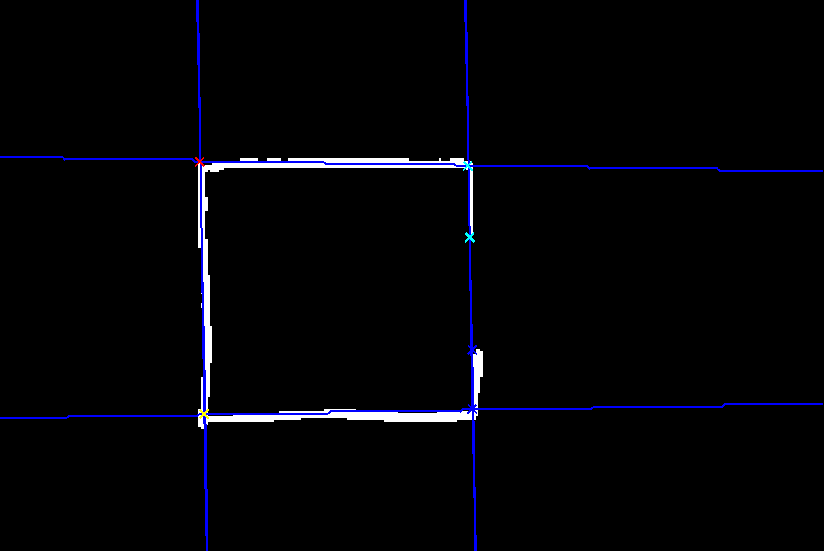
\includegraphics[scale=0.30]{rectCoax.png}
\end{tabular}
\label{tab:gt}
\caption{The detected rectangle and its vertices in Coaxing Video}
\end{figure}


\hspace*{10pt} \section{Feature Extraction}
 Feature extraction is one of the most important parts of this project. The actions in a image sequence are represented bye the motion of the objects in the video. Therefore the motion of the objects in the video is highly dependent on the other object. To discover actions in the video, we need to get the features which are relevant to their interaction and their individual actions.\\
 \hspace*{10pt} Let the feature vector of a frame is $F = \{f_1 , f_2, \cdots, f_n\}$. Here are the features which we calculated and used different subsets of these in further works :- \\

 \subsection{Position of the Triangles : }
The interaction between the objects is highly dependent on the position of the objects. The individual position of the objects also infer their relative positions.\\
\hspace*{10pt} In object identification, we calculated the coordinates of the vertices of the triangles. From them we calculate the coordinates of the centroid of each of the triangle which is also assumed to be the position of the triangle.

\subsection{Orientation of the Triangles : }
The extent of interaction between the triangles is dependent on their relative orientation, e.g. if both the triangles are facing each other(exactly opposite orientation), then they are more likely to interact or express an action.\\
\hspace*{10pt} The orientation of the triangle is calculated by tracking the motion of the triangle. The vertex relatively aligned in the direction of the motion with respect to the centroid of the triangle is the head of the triangle. The made by the line joining the centroid with the head of the triangle is the orientation of the triangle.

\begin{figure}[h]
\center
\begin{tabular}{c}
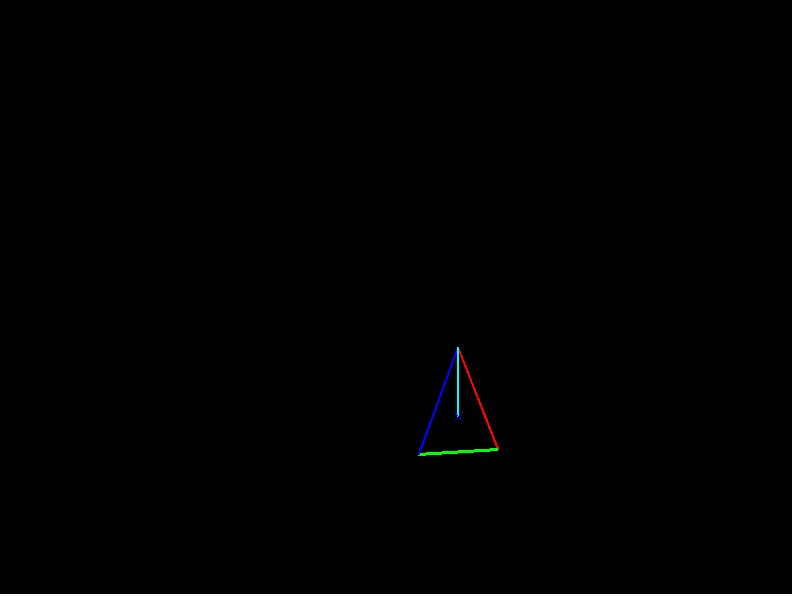
\includegraphics[scale=0.30]{orientation.png}
\end{tabular}
\label{tab:gt}
\caption{The detected rectangle and its vertices in Coaxing Video}
\end{figure}

\subsection{Visibility of the triangle :}
In the videos where the rectangular box is there, the fact that whether the two triangles are able to see each other or not and if they can then to what extent. Therefore we chose visibility too as a feature vector in the triangle.\\
\hspace*{10pt} The visibility of two triangle is a non-negative number $v \in [0, 1]$. Here $0$ means that the two triangles are completely occluded with the rectangle and $1$ means that they are completely visible to each other and any value between $0$ and $1$ is measure of extent they are visible.\\
\hspace*{10pt} The visibility of the triangles is calculated as follows :- \\
\hspace*{20pt} $1-$ Draw the supporting tangents for the two triangles. Now part of the rectangle which falls between these two lines is determined. We take the projection of this part of rectangle in directions of perpendicular to the  supported tangents is calculated. The fraction of this projection with total distance between supporting tangents is the measure of the visibility of the triangles. The figure below explains feature :- \\

\begin{figure}[h]
\center
\begin{tabular}{c}
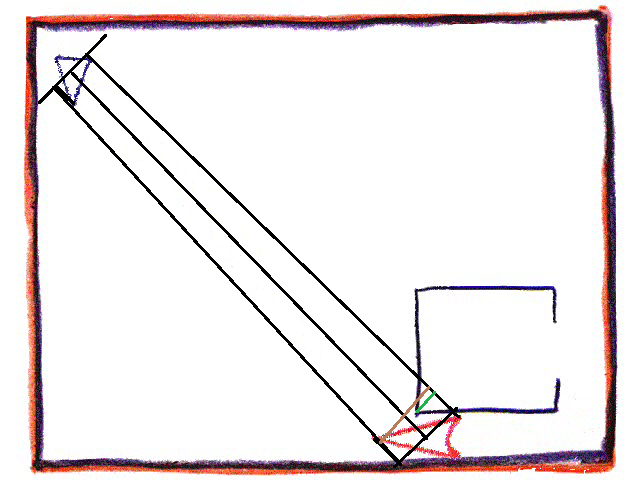
\includegraphics[scale=0.30]{visibility.png}
\end{tabular}
\label{tab:gt}
\caption{Visibility of triangles :  The brown line between the two supporting tangents is the distance between the lines and the green line is measure of occlusion and the ratio of lengths of green and brown lines is the measure of visibility}
\end{figure}

\subsection{Feature vector :}
The feature vector of a frame is a subset or derived of the previously calculated features. Let the centroid is represented by $C$ and orientation is represented by$\theta$ and the visibility between the triangles $t_1$ and $t_2$ is $v$. Then Following are some feature vector used :-\\

1- Ignore the visibility factor in both the triangles and take only the centroids and orientation of the triangles \\
\hspace*{20pt}  $\mathbf{[C_{t_1}}$ $\mathbf{C_{t_2}}$ $\mathbf{\Theta_1}$ $\mathbf{\Theta_2]}$\\
\hspace*{15pt}2- Include the visibility factor with other features\\
\hspace*{20pt} $\mathbf{[C_{t_1}}$ $\mathbf{C_{t_2}}$ $\mathbf{\Theta_1}$ $\mathbf{\Theta_2}$ $\mathbf{v]}$\\
\hspace*{15pt}3- Since $\theta$ is in $S_1$ topology, i.e it is periodic value with period $360$. It's values of $0$ and $360$ is overlapping. Therefore to remove this shortcoming, we can use the $sin$ and $cos$ of the $\theta$.\\
\hspace*{20pt} $\mathbf{[C_{t_1}}$  $\mathbf{C_{t_2}}$  $\mathbf{sin\Theta_1}$  $\mathbf{cos\Theta_1}$  $\mathbf{sin\Theta_2}$  $\mathbf{cos\Theta_2]}$\\

\hspace*{10pt} \section{Actions in the Visual Sequence :}
Actions in visual sequences are result of complicated motions of the objects in it. This complicated motion can be learnt by HMMs and appropriate feature vectors. We follow two approaches for learning the actions in the video. One is completely unsupervised hierarchical cluster based method and other is user labeled unsupervised method. These two methods differ on how we provide the input to the HMMs and how to use the created HMHs.\\

\noindent \colorbox{gray}{\rlap {\hspace*{20pt} \Large \bf A. Completely Unsupervised Method}\hspace{\linewidth}\hspace{-2\fboxsep}} 
\subsection{Learning the HMM :}

\begin{minipage}{0.4\textwidth}
\begin{flushleft} \large
We break the whole video into frame sequences each having $N$ frames and each of sequences overlap by $M$ frames. The choice of $N$ and $M$ is dependent on the approximate length of the action sequences and the time interval in which the action appears. For each of these sequence we learn HMM on that.

\end{flushleft}
\end{minipage}
\begin{minipage}{0.4\textwidth}
\begin{flushright} \large

\center
\begin{tabular}{c}
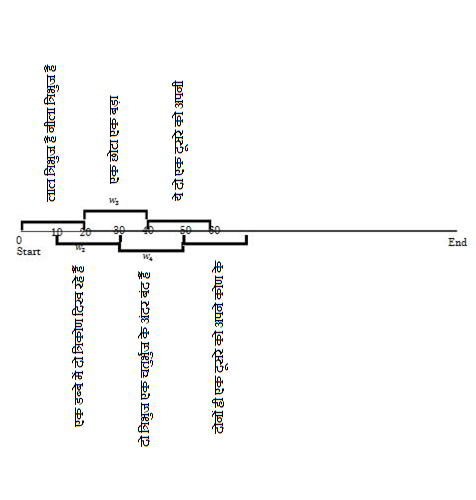
\includegraphics[scale=0.7]{interval1.png}
\end{tabular}
\label{tab:gt}

\end{flushright}
\end{minipage}\\[3cm]

\subsection{Hierarchical Clustering :}
Once we get the HMMs on all the image sequences, we calculate the distance between these HMMs. Here we take the Mutual Acceptance as the distance between to HMM. Mutual acceptance is defined as :-\\

$$dist(S_1, S_2) = \frac{|logP(S_2|\lambda _ 1)|}{N_1} +\frac{|logP(S_1|\lambda _ 2)|}{N_2} $$
Where : \\
\hspace*{20pt} $\lambda_1$ and $\lambda_2$ are HMMs trained on data $S_1$ and $S_2$ respectively.\\
\hspace*{20pt} The length of $S_1$ is $N_1$ and that of $S_2$ is $N_2$.\\

Based on this measure a hierarchical clustering is created. We used in-built function of Matlab for such clustering. A hierarchical clustering is recursively merging of clusters or points to form a single cluster in the end. Thus we get tree in which different clusters are merged at different levels based on the distance measure provided and a merging method. We used Mutual acceptance as calculated above as the distance measure and 'ward' method for merging clusters.

\begin{figure}[h]
\center
\begin{tabular}{c}
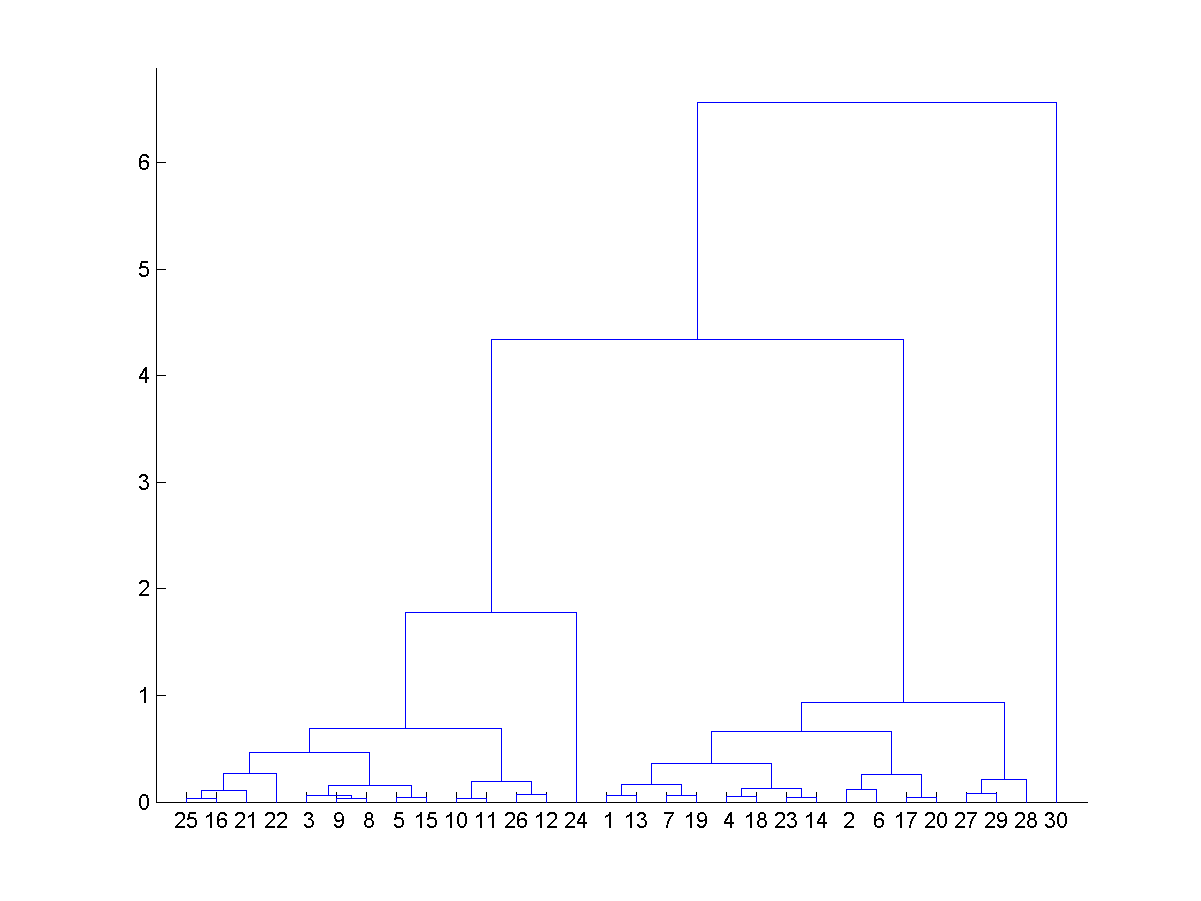
\includegraphics[scale=0.30]{dendoCoax.png}
\end{tabular}
\label{tab:gt}
\caption{The hierarchical clustering created for Coaxing video, top 30 nodes are shown}
\end{figure} 
 
 The leafs in the tree represent the individual points in the dataset while the internal nodes represent the clusters of points. The points merging near the leaves are more similar to points merging far from leaves. This hierarchical clustering helps us to classify the data into specific number of clusters. We just need to cut the tree at appropriate level for this.\\
 
\noindent \colorbox{gray}{\rlap {\hspace*{20pt} \Large \bf  B. User labeled Unsupervised Method}\hspace{\linewidth}\hspace{-2\fboxsep}} 

\subsection{Labelling the actions :}
In the Coaxing video, there are 4-5 types of actions namely {\dn \8{G}m {\rs ,\re} V\3C3wr mArnA{\rs ,\re} K\?l{\rs ,\re} lX}. Here we label all the actions and their occurrence interval in the video manually. Multiple intervals can have same actions.

\begin{figure}[h]
\center
\begin{tabular}{c}
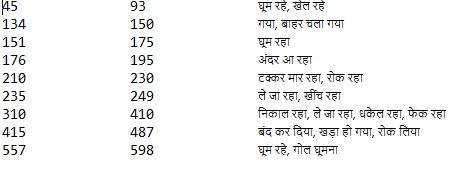
\includegraphics[scale=0.80]{userLabelActions.png}
\end{tabular}
\label{tab:gt}
\caption{User labeled actions in the Coaxing Video}
\end{figure} 

\subsection{Learning HMM on labeled actions and Merging labels:} 
In the next step we learn HMM on each of the labels. These HMMs are characteristics of the action described by that label. Now based on Mutual acceptance distance we merge the nearest HMMs. After merging we will be left with set of intervals each representing a single type of action.\\

\begin{figure}[h]
\center
\begin{tabular}{c}
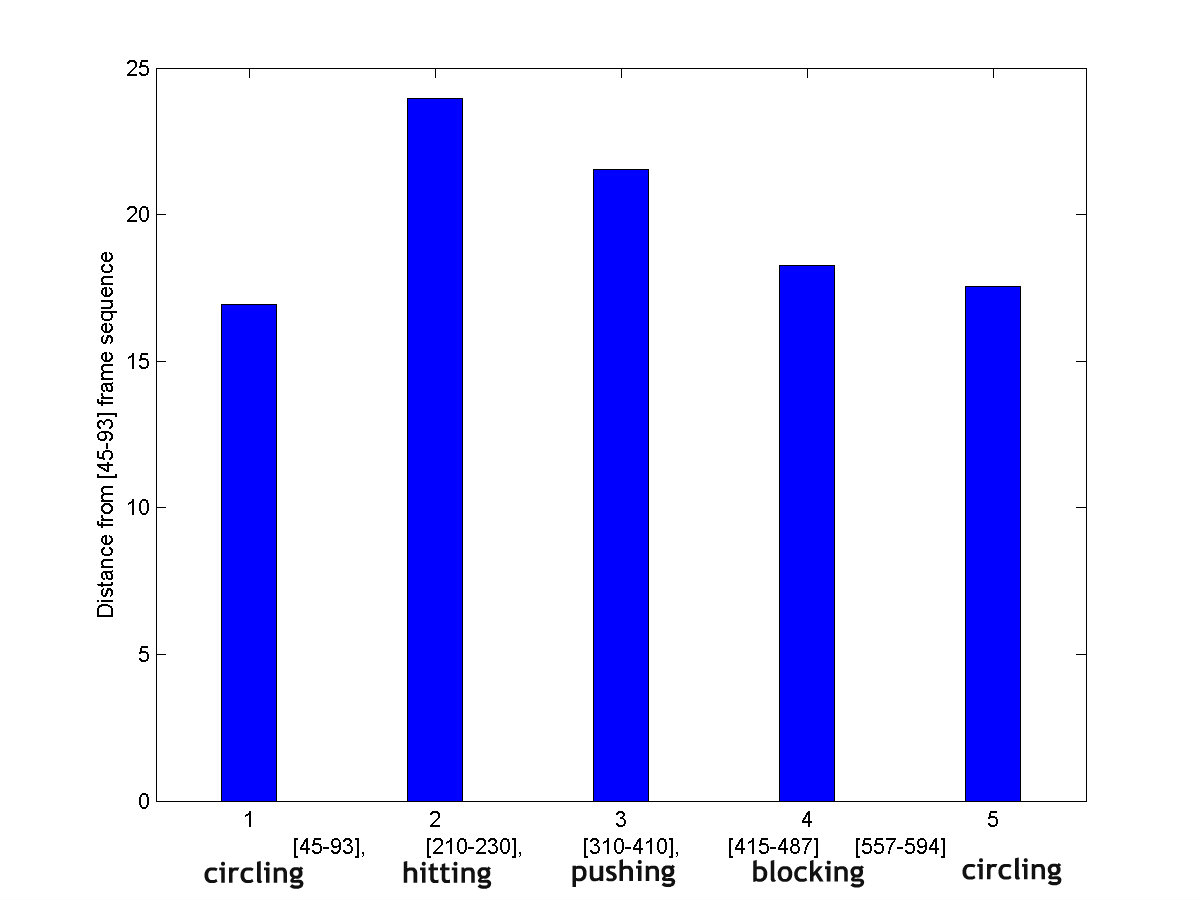
\includegraphics[scale=0.2]{barplot1.jpg}
\end{tabular}
\label{tab:gt}
\caption{HMM distances of first labeled action sequence with all other major action sequences}
\end{figure} 

%%%%%%%%%%%%%%%%%%%%%%%%%%%%%%%%%%%%%%%%%%%%%%%%%%%%%%%%%%%%%%%%%%%%%%%%%%%%%%%%
\chapter{Language Association } 
\hrule height 2pt
\vspace*{10pt} 

 Till now we are able to separate different objects in the video. Now we need to associate these objects with words. In the similar way by clustering we merge similar action and separate actions with different attributes. But we don't know how are these actions associated with the language.\\
 \hspace*{10pt} \section{Properties of Language :}
 A language has four properties :-
 \paragraph{lexicons : }
  Lexicons of a language are all the words consisting of the language. This includes all words in language and corresponding lexemes. Any sentence in a language is a subset of lexicons. To recognize the lexemes one must be able to understand the word boundaries. A child knows the words boundary very late in it's learning process\\
 \paragraph{Phonology :}
 Phonology of a language corresponds to the pronunciations in the language. Syllables of a language represent the phonological property of the language. In early learning process of child, it doesn't know the word boundaries. So it tries to map syllables to the objects and actions.
 
\paragraph{Morphology :}
The lexemes can be broken as morphemes. Morphemes are the smallest fragmentation of words which have meaning. To able to recognise the lexemes in a language one need to know the meanings of words and be able to distinguish between meaningful and meaningless syllables

\paragraph{Syntax :} 
 Syntax is structure of the sentences in a language. Syntax can be learned only with prior knowledge of lexemes, phonology and morphology of the language.\\ \\

\hspace*{10pt} Here we study only lexical and phonological properties of the language i.e syllables and words. And we don't assume any prior information about any aspect of the language. So our model will be true for any language.
%% add more text 

\section{Words Corpus :}

In the commentary, most common words of the language don't refer to the object being described. Therefore we need to remove these types of words from our commentaries.  Most common words are identified by a corpus. Below is the description of the corpus of the both language and corresponding filtering process :- \\

 \subsection{Hindi Corpus :}
 
 We use CFILT, IIT Bombay\cite{CFLIT} corpus. We calculate the absolute frequency as well as fractional frequency of each word in the corpus. Now we use two methods of filtering words from our commentaries -\\
\hspace*{10pt} {\bf 1- } We calculate the fractional frequency of each word in our commentaries. Then we remove all words in the commentary whose fractional frequency matches with that in the corpus.\\
\hspace*{10pt} {\bf 2- } We take top 1000 words in the corpus and remove them from the commentary.\\

\subsection{English Corpus :}

For English, we took most common words from DuBois Learning Center\cite{http://www.duboislc.org/EducationWatch/First100Words.html}. There are 100 most common words available here. Then we removed these words from our commentaries.\\

\section{Noun Learning :}

 Before discovering the verbs, we need to filter out the nouns in the visual sequence. Therefore we need to discover the nouns in the commentary. These nouns will primarily correspond to the moving objects and the objects more involved into the interactions. To identify the nouns, we need to build attention model :-

 \subsection{Attention Model for objects :}
 
 When any word in the commentary is said about some object in the video, we say that the object is attended.\\
	The attention model says that the subject will attend to the  objects which are moving. The subject will unlikely utter about the temporarily or permanently static object. he utters about the objects where his gaze is focused. And the gaze of human is more likely to follow the motions in a video\cite{satish-mukerjee-2008icdl}. In in a single image, the salient parts are mostly the more contrast parts and the rare or different object. But in image sequences, these factors affect the gaze much less than motion. Therefore the words in the commentary will be highly co-related to the objects which are moving in the video. Based on this assumption we identify the nouns.\\

\subsection{Determining concepts :}

Concepts play similar role in image schema as the words or syllables play  in the language. The concepts are instances of image schema. Upon hearing the utterances, it is mapped to the words which is further mapped to the concepts. Similarly on seeing the image schema, the object is being recognized and words start becoming available in symbolic unit.\\ 
\hspace*{15pt} In this project we have considered following types of concepts for noun learning :\\
\hspace*{20pt} \paragraph{(i)Concept-1} : This concept occurs when the red triangle {\bf RT} is moving and  is attended by the speaker.
\hspace*{20pt} \paragraph{(ii) Concept-2} : This concept occurs when the blue triangle {\bf BT} is moving and is attended by the speaker. 
\hspace*{20pt} \paragraph{(iii) Concept-1 Not Concept-2} : This concepts happens when the red triangle is moving and is attended, but the blue triangle is not attended by the speaker. This favors {\bf RT} strongly.
\hspace*{20pt} \paragraph{(i) Not Concept-1 Concept-2} : This concept happens when the blue triangle is moving and is attended while the red triangle is not attended by the speaker. This favors {\bf BT} strongly.
\hspace*{20pt} \paragraph{(i)Concept-1 and Concept-2} : This happens when both triangles are moving and both are attended by the speaker. This doesn't favor any object particularly.
\hspace*{20pt} \paragraph{(i) Not Concept-1 Not Concept-2} : This concept happens when none of the objects are attended in the speaker. This also doesn't favor any specific object or other aspect of the image schema.
\hspace*{15pt} We use first $4$ concepts for extracting nouns and verbs.

\subsection{Association Measures :}

Association measures are computations on the labels and visual sequences which provide the measure of co-occurrence of given label and visual sequence.\\
Given a label $l$, a concept $c$ at time $t$, following probabilities are defined :-\\
Probability that speaker $s$ has attended the concept $c$ at time $t$ is :-\\
\begin{align*}
\mathit{P(c | s, t)}  &= 1 \text{ if {\it c} is attended by speaker {\it s}  at time {\it t}} \\
   &=  0 \text{ otherwise}
\end{align*}
\begin{align*}
\mathit{P(l | s, t)}  &= 1 \text{ if {\it l} is attended by speaker {\it s}  at time {\it t}} \\
   &=  0 \text{ otherwise}
\end{align*}
	
Let's assume all the speakers are $S$ and the concepts are represented by $C$ anl the utterances are $L$. \\
Now the joint probability of the concept $c$ and utterance $l$ for all the speakers is represented as :- 
$$J(l,c) = \frac{1}{T*\|S\|} * \sum_{t =1 } ^{T}{\sum_{s\in S}{P(c|s, t) *P(l\|s, t)}}$$
Where : $T$ is total duration of the occurrence of concept \\
In the same way, the concept probability is defined : \\
$$P(c) = \frac{1}{T*\|S\|} * \sum_{t =1 } ^{T}{\sum_{s\in S}{P(c|s, t)}}$$
and label probability is : 
$$P(l) = \frac{f(l)}{\sum_l f(l)}$$
Where $f(l)$ is the frequency of label $l$ in the commentary\\
A good association measure is one which gives very high values for the labels and visual categories which co-occur frequently. It also penalize the labels which occur frequently with different visual categories. Here are some association measures used in in this project\\

\subsection{Joint Probability Results for Concepts :} Following are the results for joint probability :\\

{\bf Hindi Language : \\}
\\
\begin{center}
\begin{tabular}{||c|l||c|l||c|l||}
\hline
\multicolumn{6}{||c||}{{\bf Concept-1(Red Triangle)}}\\
\hline
\multicolumn{2}{||c||}{Monograms } &\multicolumn{2}{|c||}{Bigrams} &\multicolumn{2}{|c||}{Trigrams} \\
\hline
{\dn E/\7{B}j} & 0.245 & {\dn lAl E/\7{B}j } & 0.100 & {\dn vo CoV\? E/\7{B}j} & 0.018\\
{\dn bAhr} & 0.237 & {\dn nFlA E/\7{B}j } & 0.054 & {\dn gol gol \8{G}m} & 0.016\\
{\dn lAl } & 0.143 & {\dn CoV\? E/\7{B}j } & 0.045 & {\dn bwA E/\7{B}j bAhr} & 0.014\\
{\dn bwA} &0.124 & {\dn bAhr Dk\?l} & 0.0410 & {\dn lAl E/\7{B}j nFl\?} & 0.011\\
\hline
\end{tabular}
\captionof{table}{Joint Probability for Concept-1(Red Triangle)}
\end{center}

\begin{center}
\begin{tabular}{||c|l||c|l||c|l||}
\hline
\multicolumn{6}{||c||}{{\bf Concept-1 Not Concept-2(Red Triangle)}}\\
\hline
\multicolumn{2}{||c||}{Monograms } &\multicolumn{2}{|c||}{Bigrams} &\multicolumn{2}{|c||}{Trigrams} \\
\hline
{\dn E/\7{B}j  } & 0.034& {\dn bwA E/\7{B}j } & 0.010 & {\dn bwA E/\7{B}j CoV\? } & 0.004\\
{\dn bwA } & 0.030 & {\dn lAl E/\7{B}j } & 0.010 & {\dn E/\7{B}j CoV\? E/\7{B}j } & 0.004\\
{\dn E/koZ } & 0.029 & {\dn CoVA E/\7{B}j } & 0.009 & {\dn E/koZ CoV\? E/koZ } & 0.004\\
{\dn CoVA} &0.124 & {\dn nFlA E/\7{B}j } & 0.008 & {\dn bwA lAl E/\7{B}j } & 0.003\\
\hline
\end{tabular}
\captionof{table}{Joint Probability for Concept-1 Not Concept-2(Red Triangle)}
\end{center}


\begin{center}

\begin{tabular}{||c|l||c|l||c|l||}
\hline
\multicolumn{6}{||c||}{{\bf Concept-2(Blue Triangle)}}\\
\hline
\multicolumn{2}{||c||}{Monograms } &\multicolumn{2}{|c||}{Bigrams} &\multicolumn{2}{|c||}{Trigrams} \\
\hline
{\dn bAhr } & 0.255 & {\dn lAl E/\7{B}j } & 0.103 & {\dn lAl E/\7{B}j nFl\?} & 0.022\\
{\dn E/\7{B}j } & 0.237 & {\dn nFlA E/\7{B}j } & 0.054 & {\dn E/\7{B}j nFl\? E/\7{B}j } & 0.022\\
{\dn lAl } & 0.143 & {\dn nFl\? E/\7{B}j } & 0.045 & {\dn vo CoV\? E/\7{B}j } & 0.018\\
{\dn E/koZ} &0.124 & {\dn E/\7{B}j bAhr} & 0.0410 & {\dn lAl E/\7{B}j bAh\qq{r}} & 0.012\\
\hline
\end{tabular}
\captionof{table}{Joint Probability for Concept-2(Blue Triangle)}
\end{center}

\begin{center}

\begin{tabular}{||c|l||c|l||c|l||}
\hline
\multicolumn{6}{||c||}{\bf Not Concept-1 Concept-2(Blue Triangle) }\\
\hline
\multicolumn{2}{||c||}{Monograms } &\multicolumn{2}{|c||}{Bigrams} &\multicolumn{2}{|c||}{Trigrams} \\
\hline
{\dn E/\7{B}j } & 0.033 & {\dn nFlA E/\7{B}j } & 0.024 & {\dn nFl E/\7{B}j bAhr } & 0.008\\
{\dn bAhr } & 0.030 & {\dn lAl E/\7{B}j } & 0.014 & {\dn nFlA E/\7{B}j lAl } & 0.006\\
{\dn nFlA } & 0.024 & {\dn E/\7{B}j bAhr} & 0.011 & {\dn E/\7{B}j lAl E/\7{B}j } & 0.006\\
{\dn lAl } &0.017 & {\dn E/\7{B}j lAl} & 0.006 & {\dn nFlA E/\7{B}j a\306wdr} & 0.004\\
\hline
\end{tabular}
\captionof{table}{Joint Probability for Not Concept-1 Concept-2(Blue Triangle)}
\end{center}

%%%%%%%%%%%%%%%%%%%%%%%%%%%%%%%%%%%%%%%%%%%%%%%%ENG%%%%%%%%%%%%%%%%%%%%%%%%%%%%%%%%%%%%%%%%%%%%%%%
{\bf English Language : \\}

\begin{center}
\begin{tabular}{||c|l||c|l||c|l||}
\hline
\multicolumn{6}{||c||}{{\bf Concept-1(Red Triangle)}}\\
\hline
\multicolumn{2}{||c||}{Monograms } &\multicolumn{2}{|c||}{Bigrams} &\multicolumn{2}{|c||}{Trigrams} \\
\hline
{\bf triangle} & 0.165 & smaller triangle & 0.064 & smaller triangle outside & 0.029\\
smaller & 0.127 & {\bf bigger triangle} & 0.060 & started playing outside & 0.012\\
outside & 0.112 & small triangle & 0.032 & both started playing & 0.012\\
box & 0.104 & triangle outside & 0.029 & small object follows & 0.011\\
\hline
\end{tabular}
\captionof{table}{Joint Probability for Concept-1(Red Triangle)}
\end{center}

\begin{center}
\begin{tabular}{||c|l||c|l||c|l||}
\hline
\multicolumn{6}{||c||}{{\bf Concept-1 Not Concept-2(Red Triangle)}}\\
\hline
\multicolumn{2}{||c||}{Monograms } &\multicolumn{2}{|c||}{Bigrams} &\multicolumn{2}{|c||}{Trigrams} \\
\hline
{\bf triangles} & 0.022& basically both & 0.008 & blue smaller object & 0.006\\
box & 0.014 & smaller object & 0.006 &triangle over here & 0.003\\
{\bf triangle} & 0.010 & {\bf red object} & 0.006 & work tries move & 0.00\\
object &0.010 & blue smaller & 0.006 & within space bigger & 0.00\\
\hline
\end{tabular}
\captionof{table}{Joint Probability for Concept-1 Not Concept-2(Red Triangle)}
\end{center}


\begin{center}

\begin{tabular}{||c|l||c|l||c|l||}
\hline
\multicolumn{6}{||c||}{{\bf Concept-2(Blue Triangle)}}\\
\hline
\multicolumn{2}{||c||}{Monograms } &\multicolumn{2}{|c||}{Bigrams} &\multicolumn{2}{|c||}{Trigrams} \\
\hline
{\bf triangle }& 0.204 & {\bf smaller triangle} & 0.096 & {\bf smaller triangle outside} & 0.028\\
ouside & 0.156 & bigger triangle & 0.064 & started playing outside & 0.012\\
{\bf smaller }& 0.146 & triangle outside & 0.028 & both started playing & 0.012\\
box & 0.112 & red triangle & 0.023 & bigger triangle seems & 0.012\\
\hline
\end{tabular}
\captionof{table}{Joint Probability for Concept-2(Blue Triangle)}
\end{center}

\begin{center}

\begin{tabular}{||c|l||c|l||c|l||}
\hline
\multicolumn{6}{||c||}{\bf Not Concept-1 Concept-2(Blue Triangle) }\\
\hline
\multicolumn{2}{||c||}{Monograms } &\multicolumn{2}{|c||}{Bigrams} &\multicolumn{2}{|c||}{Trigrams} \\
\hline
{\bf triangle} & 0.036 & {\bf smaller triangle} & 0.014 & box ring basically & 0.008\\
outside & 0.031 & red triangle & 0.012 &big box ring & 0.008\\
{\bf smaller} & 0.027 & gets success & 0.009 &{\bf smaller triangle tries} & 0.005\\
box &0.016 & ring basically & 0.007 & roam around outside & 0.005\\
\hline
\end{tabular}
\captionof{table}{Joint Probability for Not Concept-1 Concept-2(Blue Triangle)}
\end{center}

\subsection{Analysis of JP Results in Both Languages :}
In all of the association measures, the single concept is weaker than the corresponding multiple concept. For example Concept-1 is weaker than Concept-1 Not Concept-2 due to obvious reasons of exclusion of the simultaneous occurrences of concepts. In the videos, most of the time both the triangles move simultaneously, therefore there is a lot of overlapping in their motion. Since we are considering words, the association of words with concept is quite discretized. So the accuracy of results varies with different measures. And sometimes, the results are unexplainable.\\

Joint probability captures the co-occurrence of the concepts and words. Following is the analysis of the result :\\
1- For  Concept-1({\bf [RT]}) and Concept-1 Not Concept-2{\bf(Strong [RT])} we get {\dn lAl E/\7{B}j} as dominating.{\bf [0.10 against 0.054]} and {\bf [0.02 against 0.017]}\\
2- For Concept-2 ({\bf [BT]}) we get {\dn lAl E/\7{B}j} as dominating.{\bf [0.103 against 0.099]}. The explanation can be given as described earlier in beginning of analysis i.e. the motions of the objects is highly overlapping and the mapping is discretized.\\
3- For Not Concept-1 Concept-2 {\bf Strong [BT]} we get {\dn nFlA E/\7{B}j} dominating.{\bf [0.024 against 0.014]}\\  
Similar analysis can be done for other English language results. For {\bf [RT]} the association in English are not very strong. But for the {\bf [BT]} the association measure are quite strong.{\bf [0.096] against [0.064]}\\
%%%%%%%%%%%%%%%%%%%%%%%%%%%%%%%%%%%%%ENG%%%%%%%%%%%%%%%%%%%%%%%%%%%%%%%%%%%%%%%%%%



\subsection{Relative Frequency :}
This measure is used in both the noun discovery as well as in verb discovery. For nouns this does not give good results because the nouns are uniformly distributed in the commentary. Relative frequency is calculated as follows :
$$RF(l,c) = \frac{\text{Frequncy of {\it l} when {\it c} is in focus}}{(\text{freq of {\it l}}) *(\text{freq of {\it l} when {\it c} is not in focus})}$$
Relative frequency gives high measures of words occurring in relatively high frequency. But it also gives high values for those words which occur seldom in the commentary. These words spoil the noun results with relative frequency measure. The solution for this is mutual information measure. 


\subsection{Mutual Information : }
Mutual information gives weight to the occurrence of a label with respect to the all words occurring for the visual sequence. Therefore it doesn't give weight to the labels seldom occurring in the commentary. Apart from that it favors, the rare concepts which co-occur with specific label frequently. And it also penalizes the words which occur most frequently with many image schema. Mutual information is defined as :- \\
 $$MI(l, c) = J(l,c)*log\left(\frac{J(l,c)}{P(c)*P(l)}\right)$$

{\bf Hindi Language Results : \\}

\begin{center}

\begin{tabular}{||c|l||c|l||c|l||}
\hline
\multicolumn{6}{||c||}{\bf Concept-1(Red Triangle) }\\
\hline
\multicolumn{2}{||c||}{Monograms } &\multicolumn{2}{|c||}{Bigrams} &\multicolumn{2}{|c||}{Trigrams} \\
\hline
{\dn E/koZ} & 0.510 & {\dn lAl E/\7{B}j} & 0.120 & {\dn vo CoV\? E/\7{B}j} & 0.042 \\
{\dn bAhr} & 0.404 &{\dn bAhr Dk\?l} & 0.117 & {\dn gol gol \8{G}m} & 0.030\\
{\dn bwA}  & 0.335 &{\dn CoV\? E/koZ} & 0.101 & {\dn dono E/\7{B}j \8{G}m } & 0.022\\
{\dn E/\7{B}j} & 0.206 & {\dn CoV\? E/\7{B}j} & 0.089 & {\dn bwA E/\7{B}j bAhr} & 0.020\\
\hline
\end{tabular}
\captionof{table}{Mutual Information results for Concept-1 (Red Triangle)}
\end{center}

\begin{center}
\begin{tabular}{||c|l||c|l||c|l||}
\hline
\multicolumn{6}{||c||}{\bf Concept-1 Not Concept-2 (Red Triangle) }\\
\hline
\multicolumn{2}{||c||}{Monograms } &\multicolumn{2}{|c||}{Bigrams} &\multicolumn{2}{|c||}{Trigrams} \\
\hline
{\dn E/koZ } & 0.158 & {\dn CoVA E/\7{B}j} & 0.025 & {\dn E/koZ CoV\? E/koZ} & 0.021\\
{\dn bwA } & 0.094 &{\dn bwA E/\7{B}j } & 0.023  & {\dn bwA E/\7{B}j CoV\? } & 0.017\\
{\dn CoVA}  & 0.065 &{\dn E/koZ CoV\? } & 0.021 & {\dn bwA lAl E/\7{B}j } & 0.014\\
{\dn tkrA} & 0.023 & {\dn CoV\? E/koZ} & 0.0206 & {\dn CoVA nFlA E/\7{B}j} & 0.012\\
\hline
\end{tabular}
\captionof{table}{Mutual Information results for Concept-1 Not Concpet-2(Red Triangle)}
\end{center}



\begin{center}
\begin{tabular}{||c|l||c|l||c|l||}
\hline
\multicolumn{6}{||c||}{\bf Concept-2 (Blue Triangle) }\\
\hline
\multicolumn{2}{||c||}{Monograms } &\multicolumn{2}{|c||}{Bigrams} &\multicolumn{2}{|c||}{Trigrams} \\
\hline
{\dn bAhr } & 0.448 & {\dn lAl E/\7{B}j} & 0.151 & {\dn vo CoV\? E/\7{B}j} & 0.041 \\
{\dn E/koZ} & 0.430 &{\dn bAhr Enkl } & 0.099 & {\dn E/\7{B}j nFl\? E/\7{B}j } & 0.041\\
{\dn CoV\?}  & 0.216 &{\dn CoV\? E/\7{B}j } & 0.090 & {\dn lAl E/\7{B}j nFl\? } & 0.036\\
{\dn E/\7{B}j} & 0.188 & {\dn nFl\? E/\7{B}j} & 0.0871 & {\dn dono E/EBj \8{G}m} & 0.021\\
\hline
\end{tabular}
\captionof{table}{Mutual Information results for Concept-2 (Blue Triangle)}
\end{center}

\begin{center}
\begin{tabular}{||c|l||c|l||c|l||}
\hline
\multicolumn{6}{||c||}{\bf Not Concept-1 Concept-2 (Blue Triangle) }\\
\hline
\multicolumn{2}{||c||}{Monograms } &\multicolumn{2}{|c||}{Bigrams} &\multicolumn{2}{|c||}{Trigrams} \\
\hline
{\dn nFl } & 0.050 & {\dn nFlA E/\7{B}j} & 0.055 & {\dn nFlA E/\7{B}j bAhr } & 0.034 \\
{\dn bAhr } & 0.037 &{\dn a\306wdr nA} & 0.018 & {\dn nFlA E/\7{B}j Upr} & 0.012\\
{\dn koE-h-h}  & 0.032 &{\dn lAl E/\7{B}j } & 0.013 & {\dn E/\7{B}j a\306wdr nA } & 0.012\\
{\dn a\306wdr} & 0.028 & {\dn vo bAhr } & 0.013 & {\dn nFlA E/\7{B}j lAl} & 0.012\\
\hline
\end{tabular}
\captionof{table}{Mutual Information results for Not Concept-1 Concept-2 (Blue Triangle)}
\end{center}


{\bf English Language Results : \\}

\begin{center}

\begin{tabular}{||c|l||c|l||c|l||}
\hline
\multicolumn{6}{||c||}{\bf Concept-1(Red Triangle) }\\
\hline
\multicolumn{2}{||c||}{Monograms } &\multicolumn{2}{|c||}{Bigrams} &\multicolumn{2}{|c||}{Trigrams} \\
\hline
{\bf triangle} & 0.211 & {\bf bigger triangle} & 0.094 &smaller triangle outside & 0.051 \\
trying & 0.205 &smaller triagle & 0.087 & started playing outside & 0.041\\
smaller & 0.190 &inner square & 0.072 & both started playing & 0.041\\
both & 0.180 & small triangle & 0.089 & small object follows & 0.020\\
\hline
\end{tabular}
\captionof{table}{Mutual Information results for Concept-1 (Red Triangle)}
\end{center}

\begin{center}
\begin{tabular}{||c|l||c|l||c|l||}
\hline
\multicolumn{6}{||c||}{\bf Concept-1 Not Concept-2 (Red Triangle) }\\
\hline
\multicolumn{2}{||c||}{Monograms } &\multicolumn{2}{|c||}{Bigrams} &\multicolumn{2}{|c||}{Trigrams} \\
\hline
{\bf triangles }& 0.071 & basically both & 0.047 & blue smaller object & 0.032\\
basically & 0.039 & smaller object & 0.032  & triangles over here & 0.016\\
here  & 0.036 &blue smaller & 0.032 & work tries move & 0.001\\
squares & 0.030 & squares here & 0.030 & within space bigger & 0.000\\
\hline
\end{tabular}
\captionof{table}{Mutual Information results for Concept-1 Not Concpet-2(Red Triangle)}
\end{center}



\begin{center}
\begin{tabular}{||c|l||c|l||c|l||}
\hline
\multicolumn{6}{||c||}{\bf Concept-2 (Blue Triangle) }\\
\hline
\multicolumn{2}{||c||}{Monograms } &\multicolumn{2}{|c||}{Bigrams} &\multicolumn{2}{|c||}{Trigrams} \\
\hline
{\bf triangle} & 0.324 & {\bf smaller triangle} & 0.186 & {\bf smaller triangle outside} & 0.047 \\
outside & 0.291 &bigger triangle & 0.107 & started playing outside & 0.041\\
{\bf smaller}  & 0.245 &red triangle & 0.050 & both started playing & 0.041\\
box & 0.185 & {\bf blue object} & 0.0416 & triangle outside again & 0.028\\
\hline
\end{tabular}
\captionof{table}{Mutual Information results for Concept-2 (Blue Triangle)}
\end{center}

\begin{center}
\begin{tabular}{||c|l||c|l||c|l||}
\hline
\multicolumn{6}{||c||}{\bf Not Concept-1 Concept-2 (Blue Triangle) }\\
\hline
\multicolumn{2}{||c||}{Monograms } &\multicolumn{2}{|c||}{Bigrams} &\multicolumn{2}{|c||}{Trigrams} \\
\hline
outside  & 0.070 & gets success & 0.051 & box ring basically & 0.040 \\
{\bf triangle} & 0.066 &red triangle & 0.051 & big box ring & 0.040\\
{\bf smaller}& 0.054 &ring basically & 0.040 &{\bf smaller triangle tries} & 0.029\\
success & 0.051 & cannot enter & 0.040 & roam around outside & 0.029\\
\hline
\end{tabular}
\captionof{table}{Mutual Information results for Not Concept-1 Concept-2 (Blue Triangle)}
\end{center}

\subsection{Analysis of MI Result in Both languages :}
Mutual Information captures the concepts and words occurring simultaneously and it penalizes the words which occur with many concepts. Following is the analysis of the results:\\
1- For Concept-1 {\bf [RT] } we get {\dn lAl E/\7{B}j } as strong association.{\bf [0.12 against 0.11]}\\
2- For Not Concept-1 Concept-2{\bf Strong [BT]}, we get {\dn nFlA E/\7{B}j} as strong association.{\bf 0.055 against 0.013}.\\
Similarly in English language :\\
1- For concept-1 {\bf [RT]}, we get bigger triangle as stong association.{\bf [0.094 against 0.087]}\\
The deviation of results from actual values is also due to morphological variations of words in Hindi.\\

\hspace*{10pt} \section{Verb Learning }
%\colorbox{gray}{\Large \bf A. Completely Unsupervised Method}\\
\subsection{Completely Unsupervised Method}
Here we get labels for the action clusters generated by hierarchical clustering. Since these clusters have larger distance between them as compared to the distances between their subsets, they are assumed to represent separate action. Therefore each cluster is treated as a separate concept. Now for labels in each concept we calculate the relative frequency measure. After ranking the values in decreasing order, we get that top-most values have labels mostly verbs, rare words and some of nouns. Here we don't get nouns because nouns are uniformly distributed in all the clusters.\\
We filter out top labels based on some threshold. Now we do more filtering by Hindi 	corpus and previously determined nouns. After this process, we majorly get the verbs for each cluster. In a cluster, verbs with highest measure and with synonyms of high measures are the action labels of the the cluster.\\\\
\subsection{Verb Learning Results :}

{\bf Hindi Language :\\}

\begin{center}
\captionof{table}{Hindi language results}
\begin{tabular}{||c|p{5cm}||p{6cm}||}
\hline
\multicolumn{1}{||c|}{Intervals } &\multicolumn{1}{|c||}{Exptected} &\multicolumn{1}{|c||}{Detected Verbs} \\
\hline
190-255 &{\dn aAnA {\rs ,\re}VkrAnA} & {\dn EBwA{\rs ,\re} Ehck{\rs ,\re} EnkAlnA{\rs ,\re}EcY{\rs ,\re} -hrmA{\rs ,\re} KF{\qva}cn\?{\rs ,\re}} {\bf{\dn V\3C3wrmArn\?}}\\
\hline
150-195 & {\dn \8{G}mnA{\rs ,\re} aAnA} & {\dn XrtA{\rs ,\re} K\?lnA{\rs ,\re} \8{G}m\?{\rs ,\re}}{\bf {\dn \8{G}mt\?}}\\
\hline
520-595	& {\dn \8{G}mnA} & {\dn vAps}\\
\hline
370-405 &{\dn D\3C3wA} & \\
\hline
400-455, 460-515 & {\dn b\2d krnA} &{\dn \7{y}D} \\
\hline
\end{tabular}
\end{center}

{\bf English Language :\\}
\begin{center}
\captionof{table}{English language results}
\begin{tabular}{||c|p{3cm}||p{8cm}||}
\hline
\multicolumn{1}{||c|}{Intervals } &\multicolumn{1}{|c||}{Exptected} &\multicolumn{1}{|c||}{Detected Verbs} \\
\hline
190-255 & Come, Hit & {\bf Coming}, Rotating, Refusing, {\bf Came}, Corner, Back, Ways, Funny, Pull, Turn, Follows\\
\hline
150-195 & Rotate, Come& Cut,{\bf Dancing}, Separated, Vertex, Chasing, Attached, Game, Side, Gone:0.67\\
\hline
520-595	&Circle, Rotate & Exploring, Interacting, Fighting, Surroundings, Also, Touched, Enjoying, Over, Happy, acquainted, Forcing, {\bf Circling, Playing:0.67} \\
\hline
370-405 & Push & Win, Drag, Here, Ahead, {\bf Pushing:0.75}\\
\hline
400-455, 460-515 & Block &Force, Forcefully, Enter, Move, {\bf Blocks}, Ring, Size, Slowly, Taunt, Explore, Roam, Push:0.67  \\
\hline
\end{tabular}
\end{center}

%\colorbox{gray}{\Large \bf B. User labeled Unsupervised Method}\\
\subsection{User labeled Unsupervised Method}
We use similar method for learning the verbs in user labeled action clusters as used for hierarchical cluster based action cluster.
Each of the clustered intervals are treated as separate concepts. Now for labels each concept, we calculate the relative frequency measure. Here again we get most verbs, rare words and some nouns as top words. Then we filter words based on association measure value, corpus and previously calculated nouns. After that we get the verbs as labels for the cluster. We compare this with the user labeled values for accuracy of results.\\

{\bf Hindi Language: \\}
\begin{center}
\captionof{table}{Verb results on user labeled clusters in Hindi}
\begin{tabular}{||c|p{5cm}||p{6cm}||}
\hline
\multicolumn{1}{||c|}{Intervals } &\multicolumn{1}{|c||}{Ground Truth } &\multicolumn{1}{|c||}{Detected Verbs} \\
\hline
45-93, 151-175, 557-198 & {\dn \8{G}m rh\?{\rs ,\re} K\?l rh\?{\rs ,\re}gol \8{G}m} & {\dn \7{K}-h{\rs ,\re} pkw{\rs ,\re} gol{\rs ,\re} \8{G}m {\rs ,\re} koZ dono{\rs ,\re} do-t}\\
\hline
134-150 & {\dn gyA{\rs ,\re} bhr clA gy} & {\dn \8{G}m\?}\\
\hline
176-195	& {\dn a\306wdr aA rhA} & {\dn vAps}\\
\hline
210-230 & {\dn V\3C3wr mAr rhA{\rs ,\re} rok rhA } & \\
\hline
235-410 & {\dn l\? jA rhA{\rs ,\re} KF{\qva}c rhA} & \\
\hline
310-410 & {\dn EnkAl rhA{\rs ,\re} l\? jA rhA{\rs ,\re} Dk\?l rhA{\rs ,\re} \327w\?k rhA} &
{\dn EnkA\qq{l}{\rs ,\re} Dk\?l{\rs ,\re} \327w\?k{\rs ,\re} trFko{\rs ,\re} D\3C3wA{\rs ,\re} Esr\?{\rs ,\re} \7{j}X{\rs ,\re} D\3C3w\?{\rs ,\re} mArkr{\rs ,\re} CotA{\rs ,\re} a\8{D}r\?{\rs ,\re} Dk\?ln\?{\rs ,\re} c\7{t}\7{B}\0j{\rs ,\re} nFl\?}\\
\hline

415-487 & {\dn b\306wd kr ElyA{\rs ,\re} KwA ho gyA{\rs ,\re} rok ElyA} & {\dn rA-tA{\rs ,\re} bd\?{\rs ,\re} KdA{\rs ,\re} \7{y}D{\rs ,\re} drvAjA{\rs ,\re} nA{\rs ,\re} BgA{\rs ,\re} EvzD{\rs ,\re} pAy\?{\rs ,\re} pw{\rs ,\re} vo{\rs ,\re} rok}\\
\hline
\end{tabular}
\end{center}

{\bf English Language: \\}
\begin{center}
\captionof{table}{Verb results of user labeled clusters in English}
\begin{tabular}{||c|p{5cm}||p{6cm}||}
\hline
\multicolumn{1}{||c|}{Intervals } &\multicolumn{1}{|c||}{Ground Truth } &\multicolumn{1}{|c||}{Detected Verbs} \\
\hline
45-93, 151-175, 557-198 & Circle, Rotate, Play & Fighting, Playing, Interacting, {\bf Circling}, Touching,Connected, Tips, Enjoying, Align, Enclosed \\
\hline
134-150 & Go Away & Chasing, Dancing\\
\hline
176-195	& Coming & Still\\
\hline
210-230 & Hit, Stop & Funny, Ways, Corner \\
\hline
235-410 & Pull & \\
\hline
310-410 & Throw, Push & {\bf Pushing, Push}, Win, Wait, Moving, Ahead \\
\hline

415-487 & Block, Stand, Roam &{\bf Blocks, Completely, Explore, Roam,} Reason\\
\hline
\end{tabular}
\end{center}
\subsection{Comparison of Results in both Languages with Both Methods : }

{\bf Hindi : }\\
\hspace*{15pt} For completely unsupervised method, we get $2$ correct mapping for words in $5$ clusters out of $12$ detected words.\\
For user labeled cluster method, we get $11$ correct mapping for $3$ clusters out of $7$ clusters and out of $20$ detected words.\\
In the user labeled learning we were able to get the verbs for all the major clusters. We could not get words for the clusters which were so small that very less commentaries could be assigned for that.\\ For completely unsupervised learning due to impurity of clusters, we were getting less accuracy.\\\\ 
{\bf English :}\\
\hspace*{10pt} Similarly in English , for completely unsupervised method, we get  $5$ correct mapping for $5$ clusters and $7$ correct word mapping out of $40$ detected words. In English we get large variety of words, so we get large number of words even after filtering.

%%%%%%%%%%%%%%%%%%%%%%%%%%%%%%%%%%%%%%%%%%%%%%%%%%%%%%%%%%%%%%%%

\chapter{Conclusion}
\hrule height 2pt
\vspace*{10pt} 
In this project, we proposed a generalized model for identification of nouns. By this model, we can detect nouns in commentary and corresponding image schema. We further tried to discover more complex schema e.g. actions. The action discovery was also generalized for multiple languages. We followed two methods for action discovery. First is by hierarchical clustering of HMMs on different segments of image schema. We create clusters from the cluster tree resulting from hierarchical clustering. And on these clusters, we identify the verbs associating the words with these clusters and then filtering out un-necessary words. The second method involved user input in form for classifying the video into segments of importance. We then merge these clusters using HMMs to get smaller number of clusters. And use similar method applied to the previously described clusters.\\
\section{Further Work :}

\hspace*{15pt} The HMMs were not able to cluster the video into very meaningful frame sequences, therefore the verbs learnt by completely unsupervised method were not as good as that in user labeled method. We can use eye gaze data for the 'Coaxing Video' to get better accuracy in noun and verb discovery. The gaze information tells the attention point of the speaker in the video. With this information, we can know, which object is being talked about. So the notion of concepts is not only based on the attention model, but is based on real data. This increases the accuracy of the results.\\ 
\hspace*{15pt} At these stage , we have nouns for the shapes in the video and verbs for the action in the video. Since we are considering mostly transitive verbs, with this much of information, we can get the predicate of actions i.e. agents involved in the actions. In that way, the syntax of a language is learnt.\\
\hspace*{15pt} Based on the information of noun and verbs, we can discover the anaphora\cite{neema-mukerjee-10_discovering-concept-of-anaphora} in the commentary of a language.

%%%%%%%%%%%%%%%%%%%%%%%%%%%%%%%%%%%%%%%%%%%%%%%%%%%%%%%%%%%%%%%%%%%%%%%%%%%%


%%%%%%%%%% APPENDIX %%%%%%%%%%%%%%%%%%%%%%%%%%%%%%%%%%%%%
\appendix
\chapter{Hough Transform}

\hrule height 2pt
\vspace*{10pt} 

\hspace*{10pt} Given a point $(x, y)$ on a line $L$. If the distance of line from origin is $r$ and the normal to the line from origin makes $\theta$ angle from the positive $x-axis$ then, the equation of the line can be written as :-\\
$$r = x cos\theta + y sin\theta$$
For each point $(x,y)$ in the combined data of triangle we get the corresponding $(r, \theta)$ pairs for $\theta \in (-180, 180]$ at the intervals of $\theta _ 0$. In this way $(R, \Theta)$ space is created. In this space the local maxima correspond to line segments. Higher the intensity of the maxima, larger the line segment corresponding to the point.\\

\chapter{Hidden Markov Models}

\hrule height 2pt
\vspace*{10pt} 

Hidden Markov Models(HMM) are dynamic Bayesian network. HMM are modelled as certain number of hidden states and some visible state. All of these states have probabilistic dependencies and these probabilistic dependencies are the characteristics of a particular HMM. Mathematically, these are modelled as follows :-\\
$$\lambda = \{A, B, \pi \}$$
Where : 
\hspace*{20pt} $A :$ State Transition Probabilities 
\hspace*{20pt} $B :$ Observation Symbol Probabilities
\hspace*{20pt} $\pi :$ Initial Probability Distribution
Like all dynamic Bayesian networks, the value of a state in HMM depends on values of  previous $k$ states. In this project, we take $k$ as $1$. So here the value of a state depends only on the previous state

\hspace*{10pt} \section{Learning an HMM }
We initialise the probabilities of HMM with selective random values i.e $\pi$. Now given the data, these probabilities are learnt by iteration. The values of these probabilities after these iterations are the characteristics of the HMM of the data.

\hspace*{10pt} \section{Loglikelihood :}
Given a learnt HMM $\lambda $ on some data $S$, and given a test $S_0$ data we can measure the similarity of this data to the HMM. This value is represented as :- \\
$$logLik = log(P(S_0 | \lambda))$$
This value is used to measure the distances between two HMMs.\\
\hspace*{10pt} \section{Distances Between HMMs}
\label{sec:distHMM}
Let a HMM learnt on Data $S_1$ of length $T_1$ is $\lambda _1$ and that on data $S_2$ of length $T_2$ is $\lambda _ 2$. The distance between the HMMs is defined as :- \\

$$dist(S_1, S_2) = \frac{|logP(S_2|\lambda _ 1)|}{T_1} +\frac{|logP(S_1|\lambda _ 2)|}{T_2} $$
  

%%%%%%%%%% BIBLIOGRAPHY %%%%%%%%%%
\bibliographystyle{plain}
\bibliography{authorName}

\end{document}